%%%%%%%%%%%%%%%%%%%%%%%%%%%%%%%%%%%%%%%%%%%%%%%%%%%%%%%%%%%%%%%%%%%%%%%%%%%%%%%%
%2345678901234567890123456789012345678901234567890123456789012345678901234567890
%        1         2         3         4         5         6         7         8
% THESIS Chapter
\chapter{Simulation and data analysis}
\label{chap:fifth}
\ifpdf
    \graphicspath{{Chapter5/Figures/PNG/}{Chapter5/Figures/PDF/}{Chapter5/Figures/}}
\else
    \graphicspath{{Chapter5/Figures/EPS/}{Chapter5/Figures/}}
\fi

\section{Results for the first experiment}

\begin{figure}[htbp]
    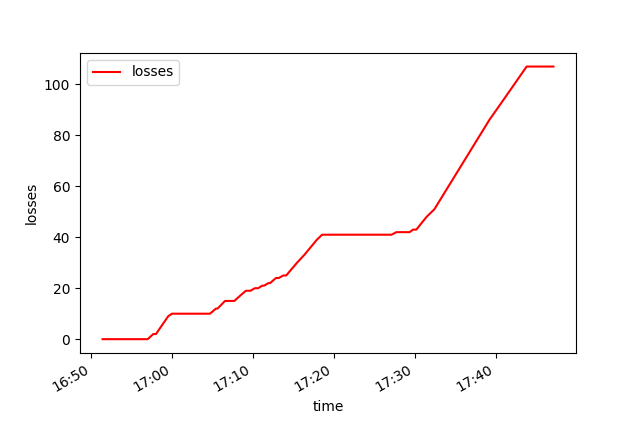
\includegraphics[width=\linewidth]{Figure_1.png}
    \caption{Acummulative packet loss with ADR depending on the time the packets arrived}
    \label{chap:fifth:fig:1}
\end{figure}

\begin{figure}[htbp]
    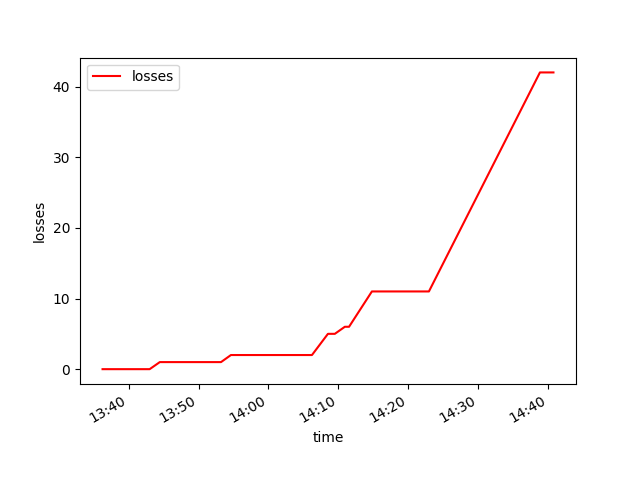
\includegraphics[width=\linewidth]{Figure_1NoADR.png}
    \caption{Acummulative packet loss without ADR depending on the time the packets arrived}
    \label{chap:fifth:fig:1:noADR}
\end{figure}

\begin{figure}[htbp]
    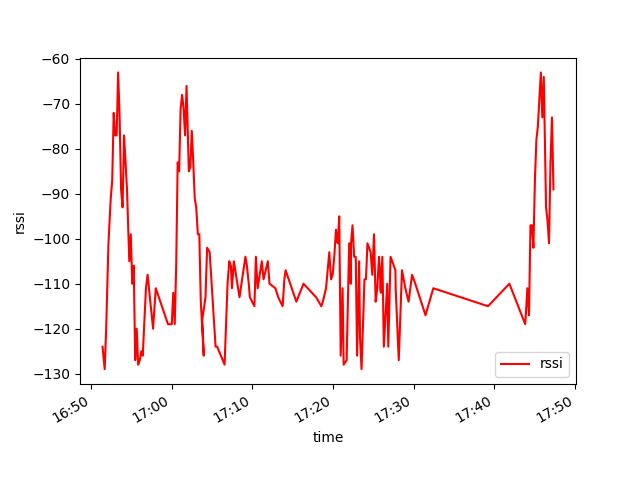
\includegraphics[width=\linewidth]{Figure_2.png}
    \caption{RSSI with ADR config. depending on the time}
    \label{chap:fifth:fig:2}
\end{figure}

\begin{figure}[htbp]
    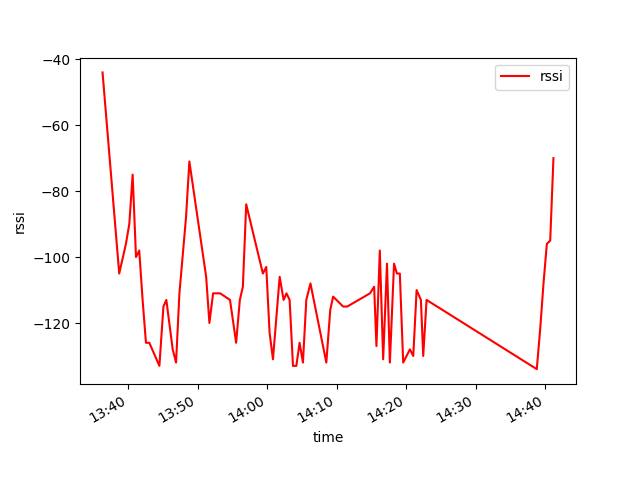
\includegraphics[width=\linewidth]{Figure_2NoADR.png}
    \caption{RSSI without ADR config. depending on the time}
    \label{chap:fifth:fig:2:noADR}
\end{figure}

\begin{figure}[htbp]
    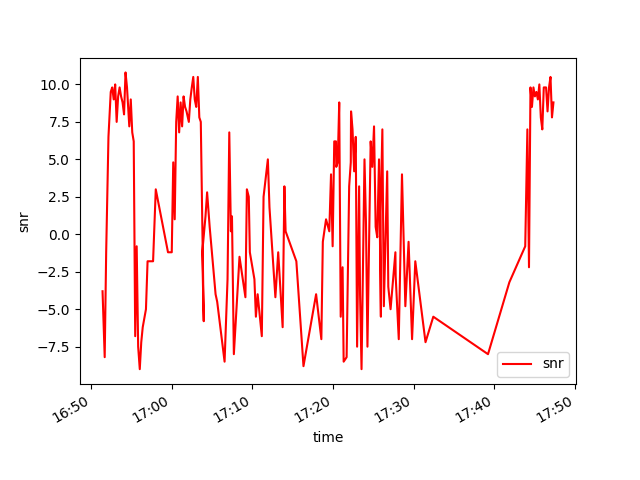
\includegraphics[width=\linewidth]{Figure_3.png}
    \caption{SNR with ADR config. depending on the time}
    \label{chap:fifth:fig:3}
\end{figure}

\begin{figure}[htbp]
    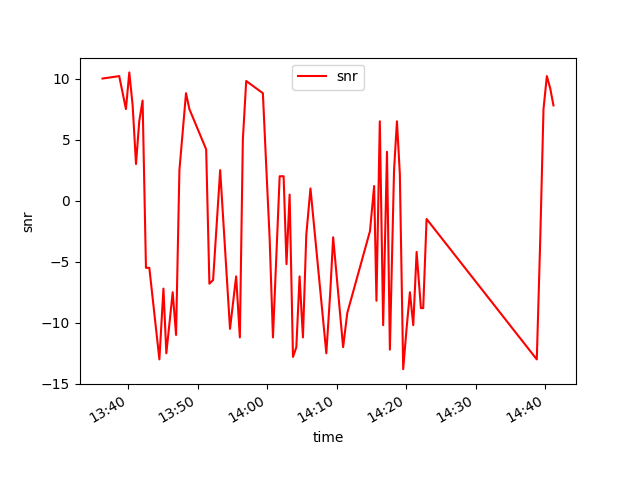
\includegraphics[width=\linewidth]{Figure_3NoADR.png}
    \caption{SNR without ADR config. depending on the time}
    \label{chap:fifth:fig:3:noADR}
\end{figure}


\begin{table}[htpb]
    \centering
    \setlength{\arrayrulewidth}{0.5mm}
    \setlength{\tabcolsep}{18pt}
    \renewcommand{\arraystretch}{2}
    \begin{tabular}{|c|c|c|c|}
        \hline
         \cellcolor[HTML]{85C1E9}ED configuration & \cellcolor[HTML]{85C1E9}Packets sent & \cellcolor[HTML]{85C1E9}Packets received & \cellcolor[HTML]{85C1E9}Packet loss\\
         \hline
         ADR activated & 263 & 156 & 40.68\% \\
         SF10 and 14 dBm & 112 & 70 & 37.5\% \\
         \hline
    \end{tabular}
    \caption{Table comparing the packet loss of the two cases}
    \label{tab:packet_loss_exp1}
\end{table}

\begin{table}[htbp]
    \centering
    \setlength{\arrayrulewidth}{0.5mm}
    \setlength{\tabcolsep}{18pt}
    \renewcommand{\arraystretch}{2}
    \begin{tabular}{|c|c|c|}
        \hline
         \cellcolor[HTML]{85C1E9}ED configuration & \cellcolor[HTML]{85C1E9}Medium SNR (dB) & \cellcolor[HTML]{85C1E9}Medium RSSI (dBm)\\
         \hline
         ADR activated & 2.07 & -103.68 \\
         SF10 and 14 dBm & -2.11 & -111.85 \\
         \hline
    \end{tabular}
    \caption{Table comparing the medium RSSI and SNR in both cases}
    \label{tab:RSSI_SNR_ex}
\end{table}